\documentclass{article}
\usepackage[left=1in, right=1in, top=1.5in, bottom=1in]{geometry}
\usepackage{fancyhdr, amsfonts, amssymb, amsthm, MnSymbol, bbm, mathrsfs, graphicx, listings, parskip, hhline}
\pagestyle{fancy}
\def\Z{\mathbb{Z}}
\def\R{\mathbb{R}}
\def\Q{\mathbb{Q}}
\def\N{\mathbb{N}}
\def\C{\mathbb{C}}
\def\P{\mathbb{P}}
\def\E{\mathbb{E}}
\def\SF{\mathscr{F}}
\def\ind{\mathbbm{1}}
\def\giv{{\,|\,}}
\def\lf{\left\lfloor}
\def\rf{\right\rfloor}
\def\lc{\left\lceil}
\def\rc{\right\rceil}
\def\eqd{ \stackrel{d}{=} }
\def\p{ \stackrel{\P}{\rightarrow} }
\def\as{ \stackrel{as}{\rightarrow} }
\def\d{ \stackrel{d}{\rightarrow} }
\def\w{ \stackrel{w}{\rightarrow} }
\def\v{ \stackrel{v}{\rightarrow} }

% 3x3 matrix code
% $$ \left( \begin{array}{ccc}
% a & b & c \\
% d & e & f \\
% g & h & i \end{array} \right)$$

% formula in array
% $$ |x| = \left\{ \begin{array}{ll}
%        x & \mbox{if $x \geq 0$};\\
%        -x & \mbox{if $x < 0$}. \end{array} \right. $$

\title{Twitter Sentiment Analysis}
\author{Eric Kim, Jonathan Wang}
\date{}

\begin{document}
\maketitle

\section{Exploratory Data Analysis}

\subsection{Data Background}
The data of interest consists of 50000 tweets with 1000 predictors of the most commonly seen words on twitter. The response is binary and tells us the sentiment of the tweet - either good or bad. We use this dataset to make predictions and submit to Kaggle. %An expanded dataset with 1.4 million tweets includes the actual tweets, and this dataset will used for feature engineering. When model fitting, we will fit and predict both with and without these features.

\subsection{Data Cleaning}
One thing to be particularly wary about is white noise in the data. In particular, these are tweets whose predictors add no value for the purposes of predictions. One example of these type of white noise tweets are those with $0$'s in each of the 1000 predictors since predicting the sentiment of the tweet with no predictors is tantamount to flipping a coin. In the smaller dataset with 50000 tweets, we find 288 of these and proceed to remove them.

Referencing the work of Pang et. al [1], we have that feature presence is more useful than feature frequency so we create a binary matrix of the initial features and compare all of the following methods with both the original data and the binary data.

Furthermore, this dataset is filled with a lot of stop word predictors. These are words that add no particular value to the predictors, that is, they amount to not much more than white noise. To reduce this white noise and speed up computation time, we use the \texttt{tm} package to remove these stop words. We further clean out the singular alphabetical letters (e.g. ``a'', ``b'', ``c'', ...). 

We also clean out the punctuation. While there are merits to including some in sentiment analysis (e.g. multiple !!!! in a row), since we binarize the data, this information is lost. However, since exclamation marks can be used in both positive and negative ways, we leave these cleaned out to avoid ambiguity. %However in the feature engineering section, we will reincorporate these features back.

Finally, we also remove any unicode characters since they too amount to white noise in the predictor set. For example, a > does not differentiate much from ? aside from the fact that in Spanish, starting a sentence with > indicates that ? will conclude the sentence or the fact that sometimes people will use > when they feel creative. 

Since we have cleaned up a lot of predictors, we are bound to have newly introduced some white noise tweets. We clean these out as well so that we end up with a compact dataset which features the most important words driving tweet sentiment and ignores as much white noise as possible.

Finally, for the sake of comparison, we will fit models on three different datasets. The full dataset with minimal cleaning of the rows with no entries in any of the predictors, the cleaned dataset as described above, and then a binarized dataset after the cleaning. These three datasets should allows us to get a good grasp on how the cleaning affected our results.

\subsection{Data Exploration}
First, we take a look at which words are most connected with positive sentiment tweets and negative sentiment tweets. To see further why we would need to clean out some of the stop words, we look at the whole data first. Of the top 50 words that showed up in the positive tweets, we see \texttt{love} 1340 times, \texttt{thanks} 1116 times, and \texttt{lol} 1058 times. Of the top 50 words after cleaning, we see \texttt{good} 1388 times, \texttt{love} 935 times, \texttt{lol} 873 times, \texttt{thanks} 649 times, \texttt{hope} 510 times, \texttt{great} 495 times, \texttt{haha} 471 times, \texttt{wish} 437 times, and \texttt{fun} 422 times. So just from a little bit of cleaning, we have retrieved more information from the data. However, one thing to note is that of the top 50, \texttt{bad} showed up 451 times and \texttt{sad} showed up 448 times. So although the words we would guess are associated with positive sentiment showed up a lot, we also find words associated with negative sentiment show up quite a bit as well.

Doing a similar analysis for the negative sentiments, we find \texttt{oh} 629 times, \texttt{miss} 534 times, \texttt{sorry} 451 times, and \texttt{sad} 429 times. However, this portion of the data is less informative since \texttt{good}, \texttt{love}, \texttt{lol}, \texttt{thanks}, \texttt{great}, \texttt{hope}, \texttt{haha}, \texttt{wish}, and \texttt{fun} all show up in the top 50. This is indicative of the fact that some words we think of as positive can also be used in a negative manner. For instance, words like \texttt{love}, \texttt{lol}, and \texttt{haha} can be used in a sarcastic tone, which often is associated with a negative context.

%\section{Feature Engineering}

\section{Hyperparameter Tuning}
For each of these methods, we use one model (typically the binarized one for the slower methods) to manually tune the hyperparameters. After finding a hyperparameter that approximately maximizes our CV Accuracy (while keeping in mind the runtime), we use this hyperparameters for all three models. And due to the limited submissions capabilities for Kaggle, we choose the models with the best CV Accuracy to submit to Kaggle and report the Kaggle Accuracy for that submission. 

\subsection{Logistic Regression}
We used \texttt{cv.glmnet} to get \texttt{lambda.min}, which is the $\lambda$ that corresponds to the lowest cross validation error. Those are reported in the next section. The following are plots of the mean cross validated error against the varying $\lambda$ values that \texttt{cv.glmnet} tried. \\

\centerline{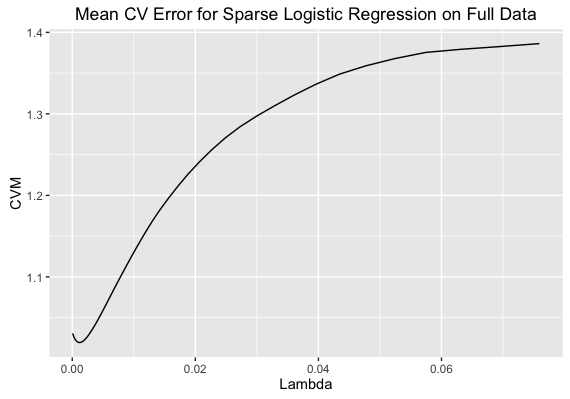
\includegraphics[scale=.3]{diagrams/1logreg.png}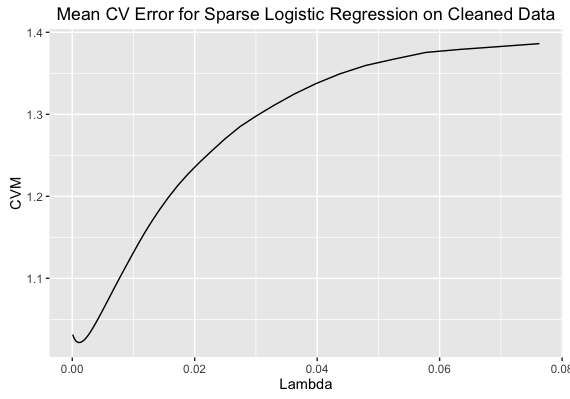
\includegraphics[scale=.3]{diagrams/2logreg.png}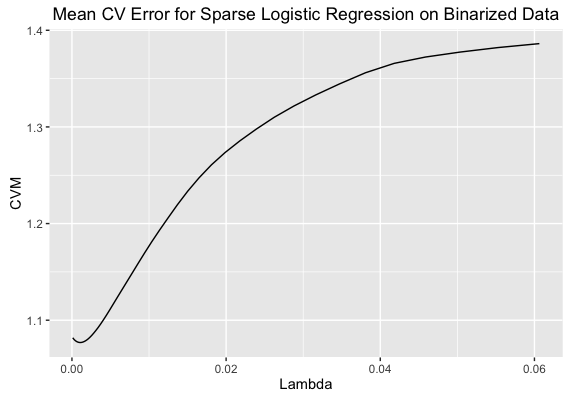
\includegraphics[scale=.3]{diagrams/3logreg.png}}

\subsection{Random Forest}

\subsection{Generalized Boosting Models}
For the GBM models, we used Adaboost with the following fixed hyperparameters \texttt{interaction.depth=5} and \texttt{shrinkage=.01}. We tried \texttt{n.trees=500,1000,1500,2000} on the binarized data. Because toward the larger tree sizes, \texttt{gbm} runs slower, we only plot out the CV Error and F1 Score (misclassification rate) against the four trees we tried. We should note that the difference between 1500 trees and 2000 trees is marginal and that any more would not give much better performance while severely overfitting. \\
\centerline{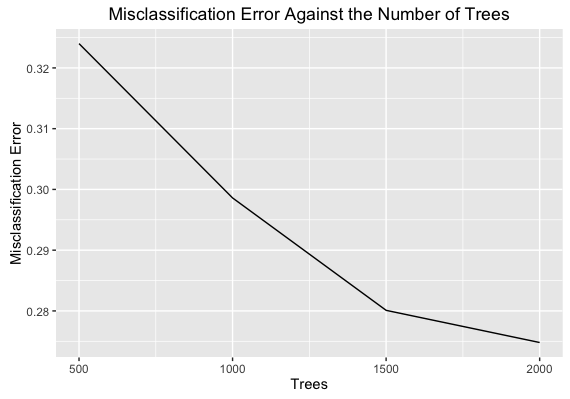
\includegraphics[scale=.35]{diagrams/4gbm.png}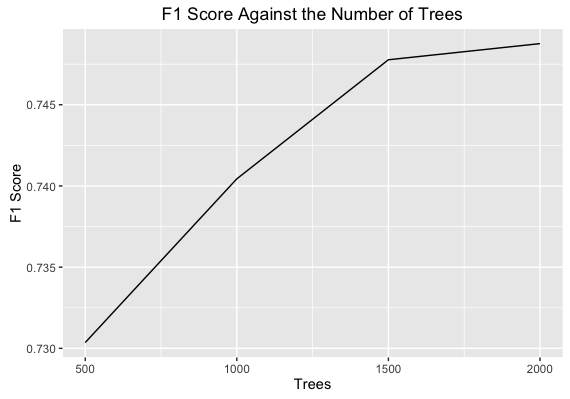
\includegraphics[scale=.35]{diagrams/5gbm.png}}

\subsection{Neural Networks}

\section{Model Fitting}
For our models, we focus on mainly four methods: logistic regression, random forest, gradient boosting, and neural networks. These models were chosen because of their natural tendencies to perform in classification. We present the results in the tables below.

\subsection{Logistic Regression}
$$\begin{array}{|c|c|c|c|c|}
\hline
\text{Model} & \text{CV Acc} & \text{Kaggle Acc} & \text{CV F1 Score} & \text{Hyper-Parameters} \\
\hhline{|=|=|=|=|=|}
\text{Logistic Regression} & 0.7576561 & 0.75844 & 0.7640936 & \lambda = 0.001153669\\
\hline
\text{Cleaned LR} & 0.732 & -- & 0.7458752 & \lambda = 0.001159524 \\
\hline
\text{Binarized LR} & 0.7314 & -- & 0.7445311 & \lambda = 0.001110128 \\
\hline
\end{array}$$
%0.7235

\subsection{Random Forest}
$$\begin{array}{|c|c|c|c|c|}
\hline
\text{Model} & \text{CV Acc} & \text{Kaggle Acc} & \text{CV F1 Score} & \text{Hyper-Parameters}   \\
\hhline{|=|=|=|=|=|}
\text{Random Forest} & 1 & 1 & 1 & \text{n.trees} = \\
\hline
\text{Cleaned RF} & 1 & 1 & 1 & \text{n.trees} = \\
\hline
\text{Binarized RF} & 1 & 1 & 1 & \text{n.trees} = \\
\hline
\end{array}$$

\subsection{Generalized Boosting Models}
$$\begin{array}{|c|c|c|c|c|}
\hline
\text{Model} & \text{CV Acc} & \text{Kaggle Acc} & \text{CV F1 Score} & \text{Hyper-Parameters} \\
\hhline{|=|=|=|=|=|}
\text{Gradient Boosting} &  &  &  & \text{n.trees} = 2000 \\
\hline
\text{Cleaned GB} &  &  &  & \text{n.trees} = 2000 \\
\hline
\text{Binarized GB} & 0.7252 & 0.70700 & 0.7487658 & \text{n.trees} = 2000 \\
\hline
\end{array}$$

\subsection{Neural Networks}
$$\begin{array}{|c|c|c|c|c|}
\hline
\text{Model} & \text{CV Acc} & \text{Kaggle Acc} & \text{CV F1 Score} & \text{Hyper-Parameters} \\
\hhline{|=|=|=|=|=|}
\text{Original Neural Networks} & 1 & 1 & 1 & 1 \\
\hline
\text{Cleaned NN} & 1 & 1 & 1 & 1 \\
\hline
\text{Binarized NN} & 1 & 1 & 1 & 1 \\
\hline
\end{array}$$

\subsection{Comparison}

\section{Ensemble Methods}
combine the methods above, probably have some sort of voting to decide new classifications (could probably do 4 different combinations of ensembles)

\subsection{[method + method]}

\subsection{[method + method + method]}

\section{Conclusion}

\section{References}
[1] Pang, B., Lee, L., Vaithyanathan, S.: Thumbs up?: sentiment classification using machine
learning techniques, pp. 79–86 (2002)
\end{document}
